\documentclass[10pt]{article}
%	options include 12pt or 11pt or 10pt
%	classes include article, report, book, letter, thesis
\usepackage[T1]{fontenc}
\usepackage[utf8]{inputenc}
\usepackage{graphicx}
\usepackage{authblk}
\usepackage{hyperref}
\usepackage{fullpage}
\usepackage{times}
\usepackage{caption}
\usepackage{wrapfig}
\usepackage{capt-of}
\newcommand{\tion}[1]{Task~\ref{#1}}
\newcommand{\fig}[1]{Fig.~\ref{#1}}

\title{\textbf{Simulation Project --- 1}}
\author{Rahul Krishna}
\affil{North Carolina State University\\Email: \href{mailto:rkrish11@ncsu.edu}{rkrish11@ncsu.edu}\thanks{Source code: \url{https://github.com/rahlk/CSC579__Computer_Performance_Modeling}}}
\date{}

\begin{document}
\maketitle
\section{Task 1}
\section{Task 2}
\section{Task 3}
\textbf{3-server Queueing System}
\begin{figure*}[ht!]
 \centering
 \begin{minipage}[]{0.33\linewidth}
  \centering
 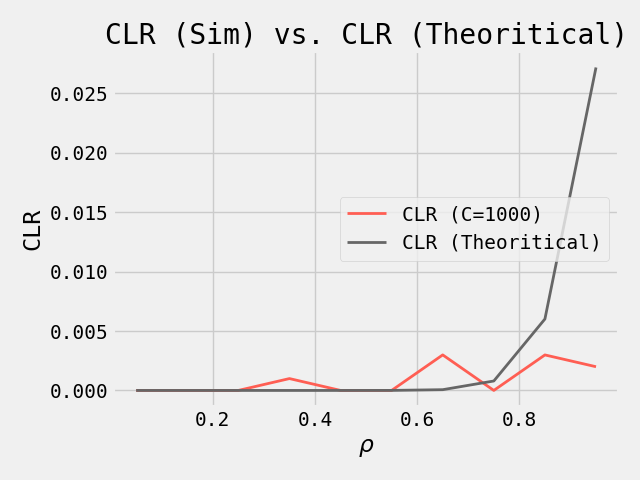
\includegraphics[width=\linewidth]{Figures/task3_1.png}
 \captionof{figure}{Customer loss rate v. $\rho$ for K=20}
 \label{fig1} 
 \end{minipage}~\begin{minipage}[]{0.33\linewidth}
  \centering
  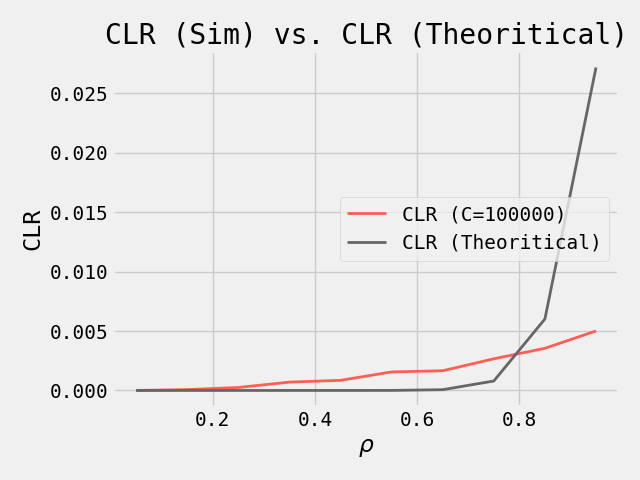
\includegraphics[width=\linewidth]{Figures/task3_2.png}
  \captionof{figure}{Customer loss rate v. $\rho$ for K=5}
  \label{fig2}
 \end{minipage}~\begin{minipage}[]{0.33\linewidth}
  \centering
  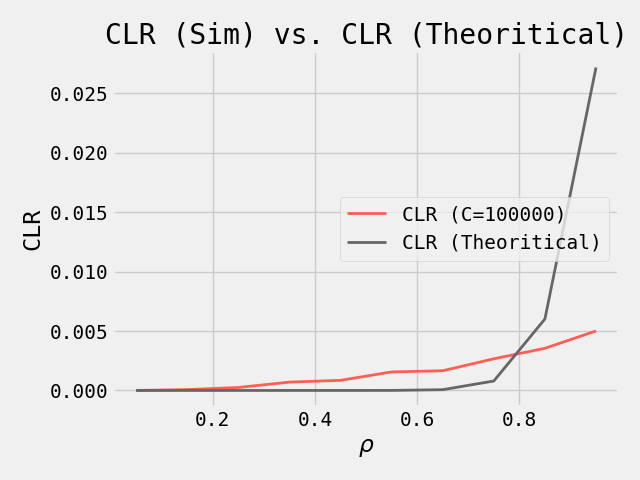
\includegraphics[width=\linewidth]{Figures/task3_2.png}
  \captionof{figure}{Customer loss rate v. $\rho$ for K=5}
  \label{fig2}
 \end{minipage}
\end{figure*}

\section{Task 4}
\textbf{1-Server Queueing System (Slowdown)}
\begin{wrapfigure}[11]{r}{0.66\linewidth}
 \centering
 \captionsetup{justification=centering}
 \begin{center}
  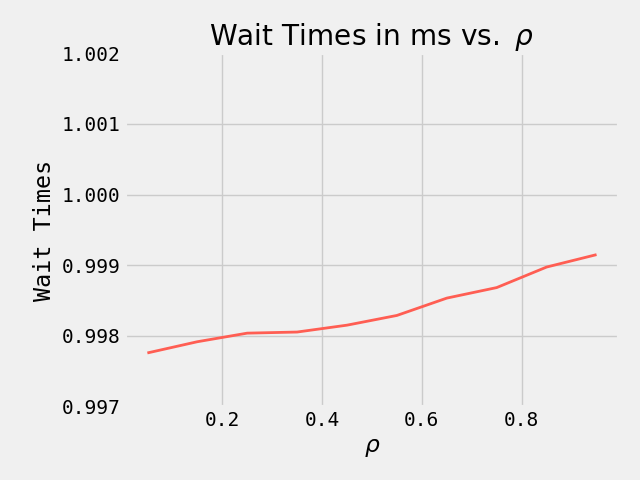
\includegraphics[width=0.8\linewidth]{Figures/task4.png}
 \end{center}
 \caption{A Plot of Wait times vs. $\rho$ for C=100000 and K=20}
 \label{fig7}
\end{wrapfigure}
\end{document}

